\documentclass[1p]{elsarticle_modified}
%\bibliographystyle{elsarticle-num}

%\usepackage[colorlinks]{hyperref}
%\usepackage{abbrmath_seonhwa} %\Abb, \Ascr, \Acal ,\Abf, \Afrak
\usepackage{amsfonts}
\usepackage{amssymb}
\usepackage{amsmath}
\usepackage{amsthm}
\usepackage{scalefnt}
\usepackage{amsbsy}
\usepackage{kotex}
\usepackage{caption}
\usepackage{subfig}
\usepackage{color}
\usepackage{graphicx}
\usepackage{xcolor} %% white, black, red, green, blue, cyan, magenta, yellow
\usepackage{float}
\usepackage{setspace}
\usepackage{hyperref}

\usepackage{tikz}
\usetikzlibrary{arrows}

\usepackage{multirow}
\usepackage{array} % fixed length table
\usepackage{hhline}

%%%%%%%%%%%%%%%%%%%%%
\makeatletter
\renewcommand*\env@matrix[1][\arraystretch]{%
	\edef\arraystretch{#1}%
	\hskip -\arraycolsep
	\let\@ifnextchar\new@ifnextchar
	\array{*\c@MaxMatrixCols c}}
\makeatother %https://tex.stackexchange.com/questions/14071/how-can-i-increase-the-line-spacing-in-a-matrix
%%%%%%%%%%%%%%%

\usepackage[normalem]{ulem}

\newcommand{\msout}[1]{\ifmmode\text{\sout{\ensuremath{#1}}}\else\sout{#1}\fi}
%SOURCE: \msout is \stkout macro in https://tex.stackexchange.com/questions/20609/strikeout-in-math-mode

\newcommand{\cancel}[1]{
	\ifmmode
	{\color{red}\msout{#1}}
	\else
	{\color{red}\sout{#1}}
	\fi
}

\newcommand{\add}[1]{
	{\color{blue}\uwave{#1}}
}

\newcommand{\replace}[2]{
	\ifmmode
	{\color{red}\msout{#1}}{\color{blue}\uwave{#2}}
	\else
	{\color{red}\sout{#1}}{\color{blue}\uwave{#2}}
	\fi
}

\newcommand{\Sol}{\mathcal{S}} %segment
\newcommand{\D}{D} %diagram
\newcommand{\A}{\mathcal{A}} %arc


%%%%%%%%%%%%%%%%%%%%%%%%%%%%%5 test

\def\sl{\operatorname{\textup{SL}}(2,\Cbb)}
\def\psl{\operatorname{\textup{PSL}}(2,\Cbb)}
\def\quan{\mkern 1mu \triangleright \mkern 1mu}

\theoremstyle{definition}
\newtheorem{thm}{Theorem}[section]
\newtheorem{prop}[thm]{Proposition}
\newtheorem{lem}[thm]{Lemma}
\newtheorem{ques}[thm]{Question}
\newtheorem{cor}[thm]{Corollary}
\newtheorem{defn}[thm]{Definition}
\newtheorem{exam}[thm]{Example}
\newtheorem{rmk}[thm]{Remark}
\newtheorem{alg}[thm]{Algorithm}

\newcommand{\I}{\sqrt{-1}}
\begin{document}

%\begin{frontmatter}
%
%\title{Boundary parabolic representations of knots up to 8 crossings}
%
%%% Group authors per affiliation:
%\author{Yunhi Cho} 
%\address{Department of Mathematics, University of Seoul, Seoul, Korea}
%\ead{yhcho@uos.ac.kr}
%
%
%\author{Seonhwa Kim} %\fnref{s_kim}}
%\address{Center for Geometry and Physics, Institute for Basic Science, Pohang, 37673, Korea}
%\ead{ryeona17@ibs.re.kr}
%
%\author{Hyuk Kim}
%\address{Department of Mathematical Sciences, Seoul National University, Seoul 08826, Korea}
%\ead{hyukkim@snu.ac.kr}
%
%\author{Seokbeom Yoon}
%\address{Department of Mathematical Sciences, Seoul National University, Seoul, 08826,  Korea}
%\ead{sbyoon15@snu.ac.kr}
%
%\begin{abstract}
%We find all boundary parabolic representation of knots up to 8 crossings.
%
%\end{abstract}
%\begin{keyword}
%    \MSC[2010] 57M25 
%\end{keyword}
%
%\end{frontmatter}

%\linenumbers
%\tableofcontents
%
\newcommand\colored[1]{\textcolor{white}{\rule[-0.35ex]{0.8em}{1.4ex}}\kern-0.8em\color{red} #1}%
%\newcommand\colored[1]{\textcolor{white}{ #1}\kern-2.17ex	\textcolor{white}{ #1}\kern-1.81ex	\textcolor{white}{ #1}\kern-2.15ex\color{red}#1	}

{\Large $\underline{12a_{0355}~(K12a_{0355})}$}

\setlength{\tabcolsep}{10pt}
\renewcommand{\arraystretch}{1.6}
\vspace{1cm}\begin{tabular}{m{100pt}>{\centering\arraybackslash}m{274pt}}
\multirow{5}{120pt}{
	\centering
	\includegraphics[width=112pt]{../../../GIT/diagram.site/Diagrams/png/1156_12a_0355.png}\\
\ \ \ A knot diagram\footnotemark}&
\allowdisplaybreaks
\textbf{Linearized knot diagam} \\
\cline{2-2}
 &
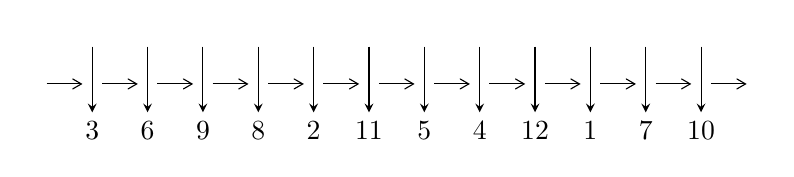
\begin{tikzpicture}[x=20pt, y=17pt]
	% nodes
	\node (C0) at (0, 0) {};
	\node (C1) at (1, 0) {};
	\node (C1U) at (1, +1) {};
	\node (C1D) at (1, -1) {3};

	\node (C2) at (2, 0) {};
	\node (C2U) at (2, +1) {};
	\node (C2D) at (2, -1) {6};

	\node (C3) at (3, 0) {};
	\node (C3U) at (3, +1) {};
	\node (C3D) at (3, -1) {9};

	\node (C4) at (4, 0) {};
	\node (C4U) at (4, +1) {};
	\node (C4D) at (4, -1) {8};

	\node (C5) at (5, 0) {};
	\node (C5U) at (5, +1) {};
	\node (C5D) at (5, -1) {2};

	\node (C6) at (6, 0) {};
	\node (C6U) at (6, +1) {};
	\node (C6D) at (6, -1) {11};

	\node (C7) at (7, 0) {};
	\node (C7U) at (7, +1) {};
	\node (C7D) at (7, -1) {5};

	\node (C8) at (8, 0) {};
	\node (C8U) at (8, +1) {};
	\node (C8D) at (8, -1) {4};

	\node (C9) at (9, 0) {};
	\node (C9U) at (9, +1) {};
	\node (C9D) at (9, -1) {12};

	\node (C10) at (10, 0) {};
	\node (C10U) at (10, +1) {};
	\node (C10D) at (10, -1) {1};

	\node (C11) at (11, 0) {};
	\node (C11U) at (11, +1) {};
	\node (C11D) at (11, -1) {7};

	\node (C12) at (12, 0) {};
	\node (C12U) at (12, +1) {};
	\node (C12D) at (12, -1) {10};
	\node (C13) at (13, 0) {};

	% arrows
	\draw[->,>={angle 60}]
	(C0) edge (C1) (C1) edge (C2) (C2) edge (C3) (C3) edge (C4) (C4) edge (C5) (C5) edge (C6) (C6) edge (C7) (C7) edge (C8) (C8) edge (C9) (C9) edge (C10) (C10) edge (C11) (C11) edge (C12) (C12) edge (C13) ;	\draw[->,>=stealth]
	(C1U) edge (C1D) (C2U) edge (C2D) (C3U) edge (C3D) (C4U) edge (C4D) (C5U) edge (C5D) (C6U) edge (C6D) (C7U) edge (C7D) (C8U) edge (C8D) (C9U) edge (C9D) (C10U) edge (C10D) (C11U) edge (C11D) (C12U) edge (C12D) ;
	\end{tikzpicture} \\
\hhline{~~} \\& 
\textbf{Solving Sequence} \\ \cline{2-2} 
 &
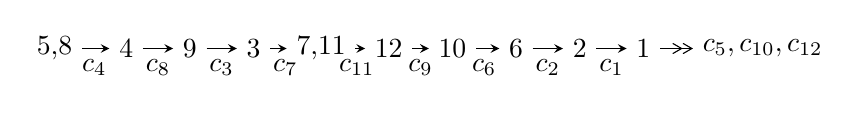
\begin{tikzpicture}[x=23pt, y=7pt]
	% node
	\node (A0) at (-1/8, 0) {5,8};
	\node (A1) at (1, 0) {4};
	\node (A2) at (2, 0) {9};
	\node (A3) at (3, 0) {3};
	\node (A4) at (65/16, 0) {7,11};
	\node (A5) at (41/8, 0) {12};
	\node (A6) at (49/8, 0) {10};
	\node (A7) at (57/8, 0) {6};
	\node (A8) at (65/8, 0) {2};
	\node (A9) at (73/8, 0) {1};
	\node (C1) at (1/2, -1) {$c_{4}$};
	\node (C2) at (3/2, -1) {$c_{8}$};
	\node (C3) at (5/2, -1) {$c_{3}$};
	\node (C4) at (7/2, -1) {$c_{7}$};
	\node (C5) at (37/8, -1) {$c_{11}$};
	\node (C6) at (45/8, -1) {$c_{9}$};
	\node (C7) at (53/8, -1) {$c_{6}$};
	\node (C8) at (61/8, -1) {$c_{2}$};
	\node (C9) at (69/8, -1) {$c_{1}$};
	\node (A10) at (11, 0) {$c_{5},c_{10},c_{12}$};

	% edge
	\draw[->,>=stealth]	
	(A0) edge (A1) (A1) edge (A2) (A2) edge (A3) (A3) edge (A4) (A4) edge (A5) (A5) edge (A6) (A6) edge (A7) (A7) edge (A8) (A8) edge (A9) ;
	\draw[->>,>={angle 60}]	
	(A9) edge (A10);
\end{tikzpicture} \\ 

\end{tabular} \\

\footnotetext{
The image of knot diagram is generated by the software ``\textbf{Draw programme}" developed by Andrew Bartholomew(\url{http://www.layer8.co.uk/maths/draw/index.htm\#Running-draw}), where we modified some parts for our purpose(\url{https://github.com/CATsTAILs/LinksPainter}).
}\phantom \\ \newline 
\centering \textbf{Ideals for irreducible components\footnotemark of $X_{\text{par}}$} 
 
\begin{align*}
I^u_{1}&=\langle 
8.94586\times10^{64} u^{73}-2.69400\times10^{64} u^{72}+\cdots+1.31582\times10^{66} b+4.80004\times10^{66},\\
\phantom{I^u_{1}}&\phantom{= \langle  }5.16081\times10^{65} u^{73}+2.32979\times10^{65} u^{72}+\cdots+1.31582\times10^{66} a-4.81901\times10^{66},\;u^{74}+2 u^{73}+\cdots-20 u-4\rangle \\
I^u_{2}&=\langle 
2 u^4-3 u^3+8 u^2+3 b-7 u+5,\;2 u^4-3 u^3+8 u^2+3 a-7 u+5,\;u^5- u^4+4 u^3-3 u^2+3 u-1\rangle \\
I^u_{3}&=\langle 
- a u+11 b-8 a+4 u-1,\;2 a^2+a u-2 a+7 u+9,\;u^2+2\rangle \\
\\
I^v_{1}&=\langle 
a,\;b+v+2,\;v^2+3 v+1\rangle \\
\end{align*}
\raggedright * 4 irreducible components of $\dim_{\mathbb{C}}=0$, with total 85 representations.\\
\footnotetext{All coefficients of polynomials are rational numbers. But the coefficients are sometimes approximated in decimal forms when there is not enough margin.}
\newpage
\renewcommand{\arraystretch}{1}
\centering \section*{I. $I^u_{1}= \langle 8.95\times10^{64} u^{73}-2.69\times10^{64} u^{72}+\cdots+1.32\times10^{66} b+4.80\times10^{66},\;5.16\times10^{65} u^{73}+2.33\times10^{65} u^{72}+\cdots+1.32\times10^{66} a-4.82\times10^{66},\;u^{74}+2 u^{73}+\cdots-20 u-4 \rangle$}
\flushleft \textbf{(i) Arc colorings}\\
\begin{tabular}{m{7pt} m{180pt} m{7pt} m{180pt} }
\flushright $a_{5}=$&$\begin{pmatrix}1\\0\end{pmatrix}$ \\
\flushright $a_{8}=$&$\begin{pmatrix}0\\u\end{pmatrix}$ \\
\flushright $a_{4}=$&$\begin{pmatrix}1\\- u^2\end{pmatrix}$ \\
\flushright $a_{9}=$&$\begin{pmatrix}- u\\u^3+u\end{pmatrix}$ \\
\flushright $a_{3}=$&$\begin{pmatrix}u^2+1\\- u^4-2 u^2\end{pmatrix}$ \\
\flushright $a_{7}=$&$\begin{pmatrix}u\\u\end{pmatrix}$ \\
\flushright $a_{11}=$&$\begin{pmatrix}-0.392213 u^{73}-0.177060 u^{72}+\cdots+27.1492 u+3.66236\\-0.0679870 u^{73}+0.0204739 u^{72}+\cdots-8.72485 u-3.64795\end{pmatrix}$ \\
\flushright $a_{12}=$&$\begin{pmatrix}-0.355590 u^{73}-0.176374 u^{72}+\cdots+34.8706 u+5.46603\\-0.0313639 u^{73}+0.0211600 u^{72}+\cdots-1.00340 u-1.84428\end{pmatrix}$ \\
\flushright $a_{10}=$&$\begin{pmatrix}-0.852587 u^{73}-1.27210 u^{72}+\cdots+13.2517 u+3.41225\\0.207785 u^{73}+0.612327 u^{72}+\cdots-5.79693 u-0.899362\end{pmatrix}$ \\
\flushright $a_{6}=$&$\begin{pmatrix}1.17691 u^{73}+1.95949 u^{72}+\cdots-19.1812 u-3.66683\\-0.0813988 u^{73}-0.326325 u^{72}+\cdots-7.72533 u+0.765144\end{pmatrix}$ \\
\flushright $a_{2}=$&$\begin{pmatrix}1.04202 u^{73}+1.78916 u^{72}+\cdots-30.0854 u-4.47897\\0.0488339 u^{73}+0.413592 u^{72}+\cdots+12.6335 u+1.99163\end{pmatrix}$ \\
\flushright $a_{1}=$&$\begin{pmatrix}1.21027 u^{73}+2.52965 u^{72}+\cdots-18.7639 u-4.59000\\0.149898 u^{73}+0.645216 u^{72}+\cdots+0.284782 u-0.278393\end{pmatrix}$\\&\end{tabular}
\flushleft \textbf{(ii) Obstruction class $= -1$}\\~\\
\flushleft \textbf{(iii) Cusp Shapes $= 3.89182 u^{73}+7.30859 u^{72}+\cdots-106.915 u-60.8282$}\\~\\
\newpage\renewcommand{\arraystretch}{1}
\flushleft \textbf{(iv) u-Polynomials at the component}\newline \\
\begin{tabular}{m{50pt}|m{274pt}}
Crossings & \hspace{64pt}u-Polynomials at each crossing \\
\hline $$\begin{aligned}c_{1}\end{aligned}$$&$\begin{aligned}
&u^{74}+36 u^{73}+\cdots+9145 u+361
\end{aligned}$\\
\hline $$\begin{aligned}c_{2},c_{5}\end{aligned}$$&$\begin{aligned}
&u^{74}+4 u^{73}+\cdots+81 u+19
\end{aligned}$\\
\hline $$\begin{aligned}c_{3},c_{4},c_{7}\\c_{8}\end{aligned}$$&$\begin{aligned}
&u^{74}-2 u^{73}+\cdots+20 u-4
\end{aligned}$\\
\hline $$\begin{aligned}c_{6},c_{11}\end{aligned}$$&$\begin{aligned}
&u^{74}-2 u^{73}+\cdots+768 u-288
\end{aligned}$\\
\hline $$\begin{aligned}c_{9},c_{10},c_{12}\end{aligned}$$&$\begin{aligned}
&u^{74}-9 u^{73}+\cdots+76 u+9
\end{aligned}$\\
\hline
\end{tabular}\\~\\
\newpage\renewcommand{\arraystretch}{1}
\flushleft \textbf{(v) Riley Polynomials at the component}\newline \\
\begin{tabular}{m{50pt}|m{274pt}}
Crossings & \hspace{64pt}Riley Polynomials at each crossing \\
\hline $$\begin{aligned}c_{1}\end{aligned}$$&$\begin{aligned}
&y^{74}+12 y^{73}+\cdots-14397001 y+130321
\end{aligned}$\\
\hline $$\begin{aligned}c_{2},c_{5}\end{aligned}$$&$\begin{aligned}
&y^{74}-36 y^{73}+\cdots-9145 y+361
\end{aligned}$\\
\hline $$\begin{aligned}c_{3},c_{4},c_{7}\\c_{8}\end{aligned}$$&$\begin{aligned}
&y^{74}+86 y^{73}+\cdots-144 y+16
\end{aligned}$\\
\hline $$\begin{aligned}c_{6},c_{11}\end{aligned}$$&$\begin{aligned}
&y^{74}-42 y^{73}+\cdots-2096640 y+82944
\end{aligned}$\\
\hline $$\begin{aligned}c_{9},c_{10},c_{12}\end{aligned}$$&$\begin{aligned}
&y^{74}-71 y^{73}+\cdots+578 y+81
\end{aligned}$\\
\hline
\end{tabular}\\~\\
\newpage\flushleft \textbf{(vi) Complex Volumes and Cusp Shapes}
$$\begin{array}{c|c|c}  
\text{Solutions to }I^u_{1}& \I (\text{vol} + \sqrt{-1}CS) & \text{Cusp shape}\\
 \hline 
\begin{aligned}
u &= \phantom{-}0.607505 + 0.741468 I \\
a &= -0.183425 - 1.058720 I \\
b &= -1.40832 - 0.47940 I\end{aligned}
 & -4.07736 - 6.36026 I & \phantom{-0.000000 } 0 \\ \hline\begin{aligned}
u &= \phantom{-}0.607505 - 0.741468 I \\
a &= -0.183425 + 1.058720 I \\
b &= -1.40832 + 0.47940 I\end{aligned}
 & -4.07736 + 6.36026 I & \phantom{-0.000000 } 0 \\ \hline\begin{aligned}
u &= -0.667561 + 0.682290 I \\
a &= \phantom{-}0.256038 - 1.207670 I \\
b &= \phantom{-}1.72165 - 0.74796 I\end{aligned}
 & -6.73194 + 12.03370 I & \phantom{-0.000000 } 0 \\ \hline\begin{aligned}
u &= -0.667561 - 0.682290 I \\
a &= \phantom{-}0.256038 + 1.207670 I \\
b &= \phantom{-}1.72165 + 0.74796 I\end{aligned}
 & -6.73194 - 12.03370 I & \phantom{-0.000000 } 0 \\ \hline\begin{aligned}
u &= -0.559459 + 0.669706 I \\
a &= -0.35510 + 1.56159 I \\
b &= -1.65441 + 0.91662 I\end{aligned}
 & -0.91245 + 7.70837 I & \phantom{-0.000000 } 0 \\ \hline\begin{aligned}
u &= -0.559459 - 0.669706 I \\
a &= -0.35510 - 1.56159 I \\
b &= -1.65441 - 0.91662 I\end{aligned}
 & -0.91245 - 7.70837 I & \phantom{-0.000000 } 0 \\ \hline\begin{aligned}
u &= -0.038593 + 0.865679 I \\
a &= -0.593774 + 0.924728 I \\
b &= \phantom{-}0.028979 + 0.303137 I\end{aligned}
 & \phantom{-}2.31614 - 1.35523 I & -12.00000 + 0. I\phantom{ +0.000000I} \\ \hline\begin{aligned}
u &= -0.038593 - 0.865679 I \\
a &= -0.593774 - 0.924728 I \\
b &= \phantom{-}0.028979 - 0.303137 I\end{aligned}
 & \phantom{-}2.31614 + 1.35523 I & -12.00000 + 0. I\phantom{ +0.000000I} \\ \hline\begin{aligned}
u &= \phantom{-}0.360711 + 0.782136 I \\
a &= \phantom{-}0.797293 + 0.395622 I \\
b &= \phantom{-}0.224581 - 0.244946 I\end{aligned}
 & \phantom{-}1.68880 - 3.09277 I & \phantom{-0.000000 } 0 \\ \hline\begin{aligned}
u &= \phantom{-}0.360711 - 0.782136 I \\
a &= \phantom{-}0.797293 - 0.395622 I \\
b &= \phantom{-}0.224581 + 0.244946 I\end{aligned}
 & \phantom{-}1.68880 + 3.09277 I & \phantom{-0.000000 } 0\\
 \hline 
 \end{array}$$\newpage$$\begin{array}{c|c|c}  
\text{Solutions to }I^u_{1}& \I (\text{vol} + \sqrt{-1}CS) & \text{Cusp shape}\\
 \hline 
\begin{aligned}
u &= -0.773386 + 0.324218 I \\
a &= -0.325616 + 0.996634 I \\
b &= -1.43090 - 0.20161 I\end{aligned}
 & -7.80941 - 7.24256 I & -12.00000 + 0. I\phantom{ +0.000000I} \\ \hline\begin{aligned}
u &= -0.773386 - 0.324218 I \\
a &= -0.325616 - 0.996634 I \\
b &= -1.43090 + 0.20161 I\end{aligned}
 & -7.80941 + 7.24256 I & -12.00000 + 0. I\phantom{ +0.000000I} \\ \hline\begin{aligned}
u &= \phantom{-}0.410374 + 0.690476 I \\
a &= \phantom{-}0.079542 + 1.327180 I \\
b &= \phantom{-}1.194690 + 0.654281 I\end{aligned}
 & \phantom{-}1.22679 - 2.85228 I & -8.14859 + 5.24888 I \\ \hline\begin{aligned}
u &= \phantom{-}0.410374 - 0.690476 I \\
a &= \phantom{-}0.079542 - 1.327180 I \\
b &= \phantom{-}1.194690 - 0.654281 I\end{aligned}
 & \phantom{-}1.22679 + 2.85228 I & -8.14859 - 5.24888 I \\ \hline\begin{aligned}
u &= \phantom{-}0.514460 + 0.613164 I \\
a &= -1.102640 - 0.882328 I \\
b &= -0.253876 + 0.423223 I\end{aligned}
 & -3.73773 - 5.34029 I & -14.6182 + 6.5473 I \\ \hline\begin{aligned}
u &= \phantom{-}0.514460 - 0.613164 I \\
a &= -1.102640 + 0.882328 I \\
b &= -0.253876 - 0.423223 I\end{aligned}
 & -3.73773 + 5.34029 I & -14.6182 - 6.5473 I \\ \hline\begin{aligned}
u &= -0.436354 + 0.667310 I \\
a &= \phantom{-}0.283686 - 0.895813 I \\
b &= \phantom{-}1.52973 + 0.27951 I\end{aligned}
 & -9.67609 + 2.66695 I & -17.4503 - 3.9305 I \\ \hline\begin{aligned}
u &= -0.436354 - 0.667310 I \\
a &= \phantom{-}0.283686 + 0.895813 I \\
b &= \phantom{-}1.52973 - 0.27951 I\end{aligned}
 & -9.67609 - 2.66695 I & -17.4503 + 3.9305 I \\ \hline\begin{aligned}
u &= \phantom{-}0.382623 + 1.141660 I \\
a &= -0.409174 - 0.900128 I \\
b &= -0.604968 - 0.087795 I\end{aligned}
 & -1.49710 - 2.18136 I & \phantom{-0.000000 } 0 \\ \hline\begin{aligned}
u &= \phantom{-}0.382623 - 1.141660 I \\
a &= -0.409174 + 0.900128 I \\
b &= -0.604968 + 0.087795 I\end{aligned}
 & -1.49710 + 2.18136 I & \phantom{-0.000000 } 0\\
 \hline 
 \end{array}$$\newpage$$\begin{array}{c|c|c}  
\text{Solutions to }I^u_{1}& \I (\text{vol} + \sqrt{-1}CS) & \text{Cusp shape}\\
 \hline 
\begin{aligned}
u &= \phantom{-}0.761356 + 0.203683 I \\
a &= -0.133816 + 0.674262 I \\
b &= \phantom{-}1.153300 - 0.116691 I\end{aligned}
 & -5.69528 + 1.81465 I & -16.3182 + 0. I\phantom{ +0.000000I} \\ \hline\begin{aligned}
u &= \phantom{-}0.761356 - 0.203683 I \\
a &= -0.133816 - 0.674262 I \\
b &= \phantom{-}1.153300 + 0.116691 I\end{aligned}
 & -5.69528 - 1.81465 I & -16.3182 + 0. I\phantom{ +0.000000I} \\ \hline\begin{aligned}
u &= -0.429289 + 0.586607 I \\
a &= \phantom{-}0.16786 - 2.19168 I \\
b &= \phantom{-}1.30415 - 1.08343 I\end{aligned}
 & -2.40757 + 2.56289 I & -14.9241 - 4.9642 I \\ \hline\begin{aligned}
u &= -0.429289 - 0.586607 I \\
a &= \phantom{-}0.16786 + 2.19168 I \\
b &= \phantom{-}1.30415 + 1.08343 I\end{aligned}
 & -2.40757 - 2.56289 I & -14.9241 + 4.9642 I \\ \hline\begin{aligned}
u &= -0.638318 + 0.268989 I \\
a &= \phantom{-}0.405828 - 1.016150 I \\
b &= \phantom{-}1.49765 + 0.09427 I\end{aligned}
 & -2.09894 - 3.64746 I & -14.7101 + 4.2800 I \\ \hline\begin{aligned}
u &= -0.638318 - 0.268989 I \\
a &= \phantom{-}0.405828 + 1.016150 I \\
b &= \phantom{-}1.49765 - 0.09427 I\end{aligned}
 & -2.09894 + 3.64746 I & -14.7101 - 4.2800 I \\ \hline\begin{aligned}
u &= -0.083637 + 1.344550 I \\
a &= -0.77219 + 1.92354 I \\
b &= -0.62622 + 1.38019 I\end{aligned}
 & \phantom{-}2.73777 - 1.04981 I & \phantom{-0.000000 } 0 \\ \hline\begin{aligned}
u &= -0.083637 - 1.344550 I \\
a &= -0.77219 - 1.92354 I \\
b &= -0.62622 - 1.38019 I\end{aligned}
 & \phantom{-}2.73777 + 1.04981 I & \phantom{-0.000000 } 0 \\ \hline\begin{aligned}
u &= -0.312075 + 1.325480 I \\
a &= \phantom{-}0.811130 - 1.137160 I \\
b &= \phantom{-}0.722128 - 0.253750 I\end{aligned}
 & -2.60689 - 3.35324 I & \phantom{-0.000000 } 0 \\ \hline\begin{aligned}
u &= -0.312075 - 1.325480 I \\
a &= \phantom{-}0.811130 + 1.137160 I \\
b &= \phantom{-}0.722128 + 0.253750 I\end{aligned}
 & -2.60689 + 3.35324 I & \phantom{-0.000000 } 0\\
 \hline 
 \end{array}$$\newpage$$\begin{array}{c|c|c}  
\text{Solutions to }I^u_{1}& \I (\text{vol} + \sqrt{-1}CS) & \text{Cusp shape}\\
 \hline 
\begin{aligned}
u &= \phantom{-}0.545002 + 0.321138 I \\
a &= -0.082844 - 0.488685 I \\
b &= \phantom{-}0.990683 + 0.671822 I\end{aligned}
 & -4.59270 + 1.67311 I & -16.9582 + 0.3985 I \\ \hline\begin{aligned}
u &= \phantom{-}0.545002 - 0.321138 I \\
a &= -0.082844 + 0.488685 I \\
b &= \phantom{-}0.990683 - 0.671822 I\end{aligned}
 & -4.59270 - 1.67311 I & -16.9582 - 0.3985 I \\ \hline\begin{aligned}
u &= -0.325449 + 0.532358 I \\
a &= \phantom{-}0.59075 - 1.40862 I \\
b &= -0.224777 - 0.237458 I\end{aligned}
 & -1.49527 + 1.17529 I & -9.83671 - 1.84843 I \\ \hline\begin{aligned}
u &= -0.325449 - 0.532358 I \\
a &= \phantom{-}0.59075 + 1.40862 I \\
b &= -0.224777 + 0.237458 I\end{aligned}
 & -1.49527 - 1.17529 I & -9.83671 + 1.84843 I \\ \hline\begin{aligned}
u &= \phantom{-}0.044226 + 0.581685 I \\
a &= \phantom{-}0.42124 - 2.21522 I \\
b &= -0.434104 - 1.036480 I\end{aligned}
 & -0.913331 + 0.906579 I & -10.85003 - 0.71233 I \\ \hline\begin{aligned}
u &= \phantom{-}0.044226 - 0.581685 I \\
a &= \phantom{-}0.42124 + 2.21522 I \\
b &= -0.434104 + 1.036480 I\end{aligned}
 & -0.913331 - 0.906579 I & -10.85003 + 0.71233 I \\ \hline\begin{aligned}
u &= \phantom{-}0.08277 + 1.44936 I \\
a &= -2.31320 - 0.95840 I \\
b &= -2.80340 - 1.07180 I\end{aligned}
 & \phantom{-}1.013510 - 0.325527 I & \phantom{-0.000000 } 0 \\ \hline\begin{aligned}
u &= \phantom{-}0.08277 - 1.44936 I \\
a &= -2.31320 + 0.95840 I \\
b &= -2.80340 + 1.07180 I\end{aligned}
 & \phantom{-}1.013510 + 0.325527 I & \phantom{-0.000000 } 0 \\ \hline\begin{aligned}
u &= -0.382429 + 0.362260 I \\
a &= -0.434039 + 0.798270 I \\
b &= -1.72137 - 0.26154 I\end{aligned}
 & -3.09747 + 0.40995 I & -17.3230 - 6.9039 I \\ \hline\begin{aligned}
u &= -0.382429 - 0.362260 I \\
a &= -0.434039 - 0.798270 I \\
b &= -1.72137 + 0.26154 I\end{aligned}
 & -3.09747 - 0.40995 I & -17.3230 + 6.9039 I\\
 \hline 
 \end{array}$$\newpage$$\begin{array}{c|c|c}  
\text{Solutions to }I^u_{1}& \I (\text{vol} + \sqrt{-1}CS) & \text{Cusp shape}\\
 \hline 
\begin{aligned}
u &= \phantom{-}0.501836 + 0.000176 I \\
a &= \phantom{-}0.258344 + 0.412671 I \\
b &= -0.700497 - 0.288592 I\end{aligned}
 & -0.628535 + 0.108862 I & -11.90695 + 0.35188 I \\ \hline\begin{aligned}
u &= \phantom{-}0.501836 - 0.000176 I \\
a &= \phantom{-}0.258344 - 0.412671 I \\
b &= -0.700497 + 0.288592 I\end{aligned}
 & -0.628535 - 0.108862 I & -11.90695 - 0.35188 I \\ \hline\begin{aligned}
u &= -0.06225 + 1.50268 I \\
a &= \phantom{-}0.35254 - 2.42780 I \\
b &= \phantom{-}0.292023 - 1.218950 I\end{aligned}
 & -4.75549 + 1.52900 I & \phantom{-0.000000 } 0 \\ \hline\begin{aligned}
u &= -0.06225 - 1.50268 I \\
a &= \phantom{-}0.35254 + 2.42780 I \\
b &= \phantom{-}0.292023 + 1.218950 I\end{aligned}
 & -4.75549 - 1.52900 I & \phantom{-0.000000 } 0 \\ \hline\begin{aligned}
u &= -0.07068 + 1.52465 I \\
a &= \phantom{-}1.88422 - 0.82743 I \\
b &= \phantom{-}2.17873 - 0.30315 I\end{aligned}
 & \phantom{-}3.33353 + 1.76863 I & \phantom{-0.000000 } 0 \\ \hline\begin{aligned}
u &= -0.07068 - 1.52465 I \\
a &= \phantom{-}1.88422 + 0.82743 I \\
b &= \phantom{-}2.17873 + 0.30315 I\end{aligned}
 & \phantom{-}3.33353 - 1.76863 I & \phantom{-0.000000 } 0 \\ \hline\begin{aligned}
u &= -0.362675 + 0.286458 I \\
a &= \phantom{-}1.62379 + 2.91989 I \\
b &= -0.876997 + 0.508032 I\end{aligned}
 & -10.87560 + 0.29586 I & -20.8413 - 9.3211 I \\ \hline\begin{aligned}
u &= -0.362675 - 0.286458 I \\
a &= \phantom{-}1.62379 - 2.91989 I \\
b &= -0.876997 - 0.508032 I\end{aligned}
 & -10.87560 - 0.29586 I & -20.8413 + 9.3211 I \\ \hline\begin{aligned}
u &= -0.09170 + 1.56641 I \\
a &= \phantom{-}0.106439 + 0.604211 I \\
b &= \phantom{-}0.786542 + 0.160086 I\end{aligned}
 & \phantom{-}5.71104 + 2.67349 I & \phantom{-0.000000 } 0 \\ \hline\begin{aligned}
u &= -0.09170 - 1.56641 I \\
a &= \phantom{-}0.106439 - 0.604211 I \\
b &= \phantom{-}0.786542 - 0.160086 I\end{aligned}
 & \phantom{-}5.71104 - 2.67349 I & \phantom{-0.000000 } 0\\
 \hline 
 \end{array}$$\newpage$$\begin{array}{c|c|c}  
\text{Solutions to }I^u_{1}& \I (\text{vol} + \sqrt{-1}CS) & \text{Cusp shape}\\
 \hline 
\begin{aligned}
u &= \phantom{-}0.04751 + 1.56902 I \\
a &= \phantom{-}0.61041 + 2.24346 I \\
b &= \phantom{-}0.99106 + 1.54336 I\end{aligned}
 & \phantom{-}6.42184 + 0.33972 I & \phantom{-0.000000 } 0 \\ \hline\begin{aligned}
u &= \phantom{-}0.04751 - 1.56902 I \\
a &= \phantom{-}0.61041 - 2.24346 I \\
b &= \phantom{-}0.99106 - 1.54336 I\end{aligned}
 & \phantom{-}6.42184 - 0.33972 I & \phantom{-0.000000 } 0 \\ \hline\begin{aligned}
u &= -0.11939 + 1.57046 I \\
a &= -0.79528 + 2.64599 I \\
b &= -1.06004 + 1.80892 I\end{aligned}
 & \phantom{-}4.90324 + 4.54099 I & \phantom{-0.000000 } 0 \\ \hline\begin{aligned}
u &= -0.11939 - 1.57046 I \\
a &= -0.79528 - 2.64599 I \\
b &= -1.06004 - 1.80892 I\end{aligned}
 & \phantom{-}4.90324 - 4.54099 I & \phantom{-0.000000 } 0 \\ \hline\begin{aligned}
u &= \phantom{-}0.14833 + 1.57361 I \\
a &= \phantom{-}0.473364 - 0.025225 I \\
b &= -0.351936 - 0.410786 I\end{aligned}
 & \phantom{-}3.62172 - 7.75592 I & \phantom{-0.000000 } 0 \\ \hline\begin{aligned}
u &= \phantom{-}0.14833 - 1.57361 I \\
a &= \phantom{-}0.473364 + 0.025225 I \\
b &= -0.351936 + 0.410786 I\end{aligned}
 & \phantom{-}3.62172 + 7.75592 I & \phantom{-0.000000 } 0 \\ \hline\begin{aligned}
u &= -0.16764 + 1.59281 I \\
a &= \phantom{-}1.15342 - 2.36244 I \\
b &= \phantom{-}1.61348 - 1.60654 I\end{aligned}
 & \phantom{-}6.70349 + 10.40740 I & \phantom{-0.000000 } 0 \\ \hline\begin{aligned}
u &= -0.16764 - 1.59281 I \\
a &= \phantom{-}1.15342 + 2.36244 I \\
b &= \phantom{-}1.61348 + 1.60654 I\end{aligned}
 & \phantom{-}6.70349 - 10.40740 I & \phantom{-0.000000 } 0 \\ \hline\begin{aligned}
u &= \phantom{-}0.12065 + 1.59882 I \\
a &= -0.96141 - 1.83317 I \\
b &= -1.43763 - 1.18663 I\end{aligned}
 & \phantom{-}9.01239 - 4.83964 I & \phantom{-0.000000 } 0 \\ \hline\begin{aligned}
u &= \phantom{-}0.12065 - 1.59882 I \\
a &= -0.96141 + 1.83317 I \\
b &= -1.43763 + 1.18663 I\end{aligned}
 & \phantom{-}9.01239 + 4.83964 I & \phantom{-0.000000 } 0\\
 \hline 
 \end{array}$$\newpage$$\begin{array}{c|c|c}  
\text{Solutions to }I^u_{1}& \I (\text{vol} + \sqrt{-1}CS) & \text{Cusp shape}\\
 \hline 
\begin{aligned}
u &= -0.13360 + 1.59895 I \\
a &= -1.44072 + 0.67557 I \\
b &= -1.80299 - 0.01955 I\end{aligned}
 & -1.95351 + 4.80687 I & \phantom{-0.000000 } 0 \\ \hline\begin{aligned}
u &= -0.13360 - 1.59895 I \\
a &= -1.44072 - 0.67557 I \\
b &= -1.80299 + 0.01955 I\end{aligned}
 & -1.95351 - 4.80687 I & \phantom{-0.000000 } 0 \\ \hline\begin{aligned}
u &= -0.21190 + 1.59846 I \\
a &= -1.20844 + 2.04050 I \\
b &= -1.81241 + 1.29307 I\end{aligned}
 & \phantom{-}0.8816 + 15.3259 I & \phantom{-0.000000 } 0 \\ \hline\begin{aligned}
u &= -0.21190 - 1.59846 I \\
a &= -1.20844 - 2.04050 I \\
b &= -1.81241 - 1.29307 I\end{aligned}
 & \phantom{-}0.8816 - 15.3259 I & \phantom{-0.000000 } 0 \\ \hline\begin{aligned}
u &= \phantom{-}0.18569 + 1.61660 I \\
a &= \phantom{-}1.01642 + 1.53262 I \\
b &= \phantom{-}1.55579 + 0.86892 I\end{aligned}
 & \phantom{-}3.86130 - 9.35513 I & \phantom{-0.000000 } 0 \\ \hline\begin{aligned}
u &= \phantom{-}0.18569 - 1.61660 I \\
a &= \phantom{-}1.01642 - 1.53262 I \\
b &= \phantom{-}1.55579 - 0.86892 I\end{aligned}
 & \phantom{-}3.86130 + 9.35513 I & \phantom{-0.000000 } 0 \\ \hline\begin{aligned}
u &= -0.02145 + 1.62935 I \\
a &= \phantom{-}0.039433 - 0.379694 I \\
b &= -0.521747 - 0.073738 I\end{aligned}
 & \phantom{-}10.84750 - 1.02517 I & \phantom{-0.000000 } 0 \\ \hline\begin{aligned}
u &= -0.02145 - 1.62935 I \\
a &= \phantom{-}0.039433 + 0.379694 I \\
b &= -0.521747 + 0.073738 I\end{aligned}
 & \phantom{-}10.84750 + 1.02517 I & \phantom{-0.000000 } 0 \\ \hline\begin{aligned}
u &= \phantom{-}0.08779 + 1.62994 I \\
a &= -0.272775 + 0.123691 I \\
b &= \phantom{-}0.280139 + 0.277553 I\end{aligned}
 & \phantom{-}9.99358 - 4.73908 I & \phantom{-0.000000 } 0 \\ \hline\begin{aligned}
u &= \phantom{-}0.08779 - 1.62994 I \\
a &= -0.272775 - 0.123691 I \\
b &= \phantom{-}0.280139 - 0.277553 I\end{aligned}
 & \phantom{-}9.99358 + 4.73908 I & \phantom{-0.000000 } 0\\
 \hline 
 \end{array}$$\newpage$$\begin{array}{c|c|c}  
\text{Solutions to }I^u_{1}& \I (\text{vol} + \sqrt{-1}CS) & \text{Cusp shape}\\
 \hline 
\begin{aligned}
u &= \phantom{-}0.355126\phantom{ +0.000000I} \\
a &= \phantom{-}0.787893\phantom{ +0.000000I} \\
b &= -0.561465\phantom{ +0.000000I}\end{aligned}
 & -0.670068\phantom{ +0.000000I} & -14.5670\phantom{ +0.000000I} \\ \hline\begin{aligned}
u &= -0.273544\phantom{ +0.000000I} \\
a &= -0.903552\phantom{ +0.000000I} \\
b &= -2.51009\phantom{ +0.000000I}\end{aligned}
 & -2.88449\phantom{ +0.000000I} & -51.7460\phantom{ +0.000000I} \\ \hline\begin{aligned}
u &= \phantom{-}0.04621 + 1.72842 I \\
a &= \phantom{-}0.110542 + 0.138918 I \\
b &= \phantom{-}0.197044 - 0.248926 I\end{aligned}
 & \phantom{-}8.82291 - 3.58672 I & \phantom{-0.000000 } 0 \\ \hline\begin{aligned}
u &= \phantom{-}0.04621 - 1.72842 I \\
a &= \phantom{-}0.110542 - 0.138918 I \\
b &= \phantom{-}0.197044 + 0.248926 I\end{aligned}
 & \phantom{-}8.82291 + 3.58672 I & \phantom{-0.000000 } 0\\
 \hline 
 \end{array}$$\newpage\newpage\renewcommand{\arraystretch}{1}
\centering \section*{II. $I^u_{2}= \langle 2 u^4-3 u^3+8 u^2+3 b-7 u+5,\;2 u^4-3 u^3+8 u^2+3 a-7 u+5,\;u^5- u^4+4 u^3-3 u^2+3 u-1 \rangle$}
\flushleft \textbf{(i) Arc colorings}\\
\begin{tabular}{m{7pt} m{180pt} m{7pt} m{180pt} }
\flushright $a_{5}=$&$\begin{pmatrix}1\\0\end{pmatrix}$ \\
\flushright $a_{8}=$&$\begin{pmatrix}0\\u\end{pmatrix}$ \\
\flushright $a_{4}=$&$\begin{pmatrix}1\\- u^2\end{pmatrix}$ \\
\flushright $a_{9}=$&$\begin{pmatrix}- u\\u^3+u\end{pmatrix}$ \\
\flushright $a_{3}=$&$\begin{pmatrix}u^2+1\\- u^4-2 u^2\end{pmatrix}$ \\
\flushright $a_{7}=$&$\begin{pmatrix}u\\u\end{pmatrix}$ \\
\flushright $a_{11}=$&$\begin{pmatrix}-\frac{2}{3} u^4+u^3-\frac{8}{3} u^2+\frac{7}{3} u-\frac{5}{3}\\-\frac{2}{3} u^4+u^3-\frac{8}{3} u^2+\frac{7}{3} u-\frac{5}{3}\end{pmatrix}$ \\
\flushright $a_{12}=$&$\begin{pmatrix}-\frac{2}{3} u^4+u^3-\frac{8}{3} u^2+\frac{7}{3} u-\frac{5}{3}\\-\frac{2}{3} u^4+u^3-\frac{8}{3} u^2+\frac{7}{3} u-\frac{5}{3}\end{pmatrix}$ \\
\flushright $a_{10}=$&$\begin{pmatrix}-\frac{2}{3} u^4+u^3-\frac{8}{3} u^2+\frac{4}{3} u-\frac{5}{3}\\-\frac{2}{3} u^4+2 u^3+\cdots+\frac{10}{3} u-\frac{5}{3}\end{pmatrix}$ \\
\flushright $a_{6}=$&$\begin{pmatrix}u\\u\end{pmatrix}$ \\
\flushright $a_{2}=$&$\begin{pmatrix}u^3+2 u\\- u^4+u^3-3 u^2+2 u-1\end{pmatrix}$ \\
\flushright $a_{1}=$&$\begin{pmatrix}u\\- u^3- u\end{pmatrix}$\\&\end{tabular}
\flushleft \textbf{(ii) Obstruction class $= 1$}\\~\\
\flushleft \textbf{(iii) Cusp Shapes $= -\frac{14}{9} u^4+\frac{11}{3} u^3-\frac{77}{9} u^2+\frac{88}{9} u-\frac{137}{9}$}\\~\\
\newpage\renewcommand{\arraystretch}{1}
\flushleft \textbf{(iv) u-Polynomials at the component}\newline \\
\begin{tabular}{m{50pt}|m{274pt}}
Crossings & \hspace{64pt}u-Polynomials at each crossing \\
\hline $$\begin{aligned}c_{1},c_{3},c_{4}\end{aligned}$$&$\begin{aligned}
&u^5- u^4+4 u^3-3 u^2+3 u-1
\end{aligned}$\\
\hline $$\begin{aligned}c_{2}\end{aligned}$$&$\begin{aligned}
&u^5- u^4+u^2+u-1
\end{aligned}$\\
\hline $$\begin{aligned}c_{5}\end{aligned}$$&$\begin{aligned}
&u^5+u^4- u^2+u+1
\end{aligned}$\\
\hline $$\begin{aligned}c_{6},c_{11}\end{aligned}$$&$\begin{aligned}
&u^5
\end{aligned}$\\
\hline $$\begin{aligned}c_{7},c_{8}\end{aligned}$$&$\begin{aligned}
&u^5+u^4+4 u^3+3 u^2+3 u+1
\end{aligned}$\\
\hline $$\begin{aligned}c_{9},c_{10}\end{aligned}$$&$\begin{aligned}
&(u-1)^5
\end{aligned}$\\
\hline $$\begin{aligned}c_{12}\end{aligned}$$&$\begin{aligned}
&(u+1)^5
\end{aligned}$\\
\hline
\end{tabular}\\~\\
\newpage\renewcommand{\arraystretch}{1}
\flushleft \textbf{(v) Riley Polynomials at the component}\newline \\
\begin{tabular}{m{50pt}|m{274pt}}
Crossings & \hspace{64pt}Riley Polynomials at each crossing \\
\hline $$\begin{aligned}c_{1},c_{3},c_{4}\\c_{7},c_{8}\end{aligned}$$&$\begin{aligned}
&y^5+7 y^4+16 y^3+13 y^2+3 y-1
\end{aligned}$\\
\hline $$\begin{aligned}c_{2},c_{5}\end{aligned}$$&$\begin{aligned}
&y^5- y^4+4 y^3-3 y^2+3 y-1
\end{aligned}$\\
\hline $$\begin{aligned}c_{6},c_{11}\end{aligned}$$&$\begin{aligned}
&y^5
\end{aligned}$\\
\hline $$\begin{aligned}c_{9},c_{10},c_{12}\end{aligned}$$&$\begin{aligned}
&(y-1)^5
\end{aligned}$\\
\hline
\end{tabular}\\~\\
\newpage\flushleft \textbf{(vi) Complex Volumes and Cusp Shapes}
$$\begin{array}{c|c|c}  
\text{Solutions to }I^u_{2}& \I (\text{vol} + \sqrt{-1}CS) & \text{Cusp shape}\\
 \hline 
\begin{aligned}
u &= \phantom{-}0.233677 + 0.885557 I \\
a &= \phantom{-}0.046507 + 0.815869 I \\
b &= \phantom{-}0.046507 + 0.815869 I\end{aligned}
 & \phantom{-}0.17487 - 2.21397 I & -9.22580 + 4.04289 I \\ \hline\begin{aligned}
u &= \phantom{-}0.233677 - 0.885557 I \\
a &= \phantom{-}0.046507 - 0.815869 I \\
b &= \phantom{-}0.046507 - 0.815869 I\end{aligned}
 & \phantom{-}0.17487 + 2.21397 I & -9.22580 - 4.04289 I \\ \hline\begin{aligned}
u &= \phantom{-}0.416284\phantom{ +0.000000I} \\
a &= -1.10533\phantom{ +0.000000I} \\
b &= -1.10533\phantom{ +0.000000I}\end{aligned}
 & -2.52712\phantom{ +0.000000I} & -12.4170\phantom{ +0.000000I} \\ \hline\begin{aligned}
u &= \phantom{-}0.05818 + 1.69128 I \\
a &= \phantom{-}0.172825 - 0.649395 I \\
b &= \phantom{-}0.172825 - 0.649395 I\end{aligned}
 & \phantom{-}9.31336 - 3.33174 I & -4.67696 - 1.07305 I \\ \hline\begin{aligned}
u &= \phantom{-}0.05818 - 1.69128 I \\
a &= \phantom{-}0.172825 + 0.649395 I \\
b &= \phantom{-}0.172825 + 0.649395 I\end{aligned}
 & \phantom{-}9.31336 + 3.33174 I & -4.67696 + 1.07305 I\\
 \hline 
 \end{array}$$\newpage\newpage\renewcommand{\arraystretch}{1}
\centering \section*{III. $I^u_{3}= \langle - a u+11 b-8 a+4 u-1,\;2 a^2+a u-2 a+7 u+9,\;u^2+2 \rangle$}
\flushleft \textbf{(i) Arc colorings}\\
\begin{tabular}{m{7pt} m{180pt} m{7pt} m{180pt} }
\flushright $a_{5}=$&$\begin{pmatrix}1\\0\end{pmatrix}$ \\
\flushright $a_{8}=$&$\begin{pmatrix}0\\u\end{pmatrix}$ \\
\flushright $a_{4}=$&$\begin{pmatrix}1\\2\end{pmatrix}$ \\
\flushright $a_{9}=$&$\begin{pmatrix}- u\\- u\end{pmatrix}$ \\
\flushright $a_{3}=$&$\begin{pmatrix}-1\\0\end{pmatrix}$ \\
\flushright $a_{7}=$&$\begin{pmatrix}u\\u\end{pmatrix}$ \\
\flushright $a_{11}=$&$\begin{pmatrix}a\\0.0909091 a u+0.727273 a-0.363636 u+0.0909091\end{pmatrix}$ \\
\flushright $a_{12}=$&$\begin{pmatrix}0.181818 a u+0.454545 a-0.727273 u+0.181818\\0.272727 a u+0.181818 a-1.09091 u+0.272727\end{pmatrix}$ \\
\flushright $a_{10}=$&$\begin{pmatrix}-0.0909091 a u+0.272727 a-1.13636 u+0.909091\\-0.181818 a u+0.545455 a-0.272727 u+0.818182\end{pmatrix}$ \\
\flushright $a_{6}=$&$\begin{pmatrix}0.0909091 a u-0.272727 a-0.863636 u+1.09091\\1\end{pmatrix}$ \\
\flushright $a_{2}=$&$\begin{pmatrix}0.0909091 a u-0.272727 a-0.863636 u+0.0909091\\1\end{pmatrix}$ \\
\flushright $a_{1}=$&$\begin{pmatrix}0.0909091 a u-0.272727 a-0.863636 u+1.09091\\1\end{pmatrix}$\\&\end{tabular}
\flushleft \textbf{(ii) Obstruction class $= 1$}\\~\\
\flushleft \textbf{(iii) Cusp Shapes $= -16$}\\~\\
\newpage\renewcommand{\arraystretch}{1}
\flushleft \textbf{(iv) u-Polynomials at the component}\newline \\
\begin{tabular}{m{50pt}|m{274pt}}
Crossings & \hspace{64pt}u-Polynomials at each crossing \\
\hline $$\begin{aligned}c_{1},c_{5}\end{aligned}$$&$\begin{aligned}
&(u-1)^4
\end{aligned}$\\
\hline $$\begin{aligned}c_{2}\end{aligned}$$&$\begin{aligned}
&(u+1)^4
\end{aligned}$\\
\hline $$\begin{aligned}c_{3},c_{4},c_{7}\\c_{8}\end{aligned}$$&$\begin{aligned}
&(u^2+2)^2
\end{aligned}$\\
\hline $$\begin{aligned}c_{6},c_{12}\end{aligned}$$&$\begin{aligned}
&(u^2- u-1)^2
\end{aligned}$\\
\hline $$\begin{aligned}c_{9},c_{10},c_{11}\end{aligned}$$&$\begin{aligned}
&(u^2+u-1)^2
\end{aligned}$\\
\hline
\end{tabular}\\~\\
\newpage\renewcommand{\arraystretch}{1}
\flushleft \textbf{(v) Riley Polynomials at the component}\newline \\
\begin{tabular}{m{50pt}|m{274pt}}
Crossings & \hspace{64pt}Riley Polynomials at each crossing \\
\hline $$\begin{aligned}c_{1},c_{2},c_{5}\end{aligned}$$&$\begin{aligned}
&(y-1)^4
\end{aligned}$\\
\hline $$\begin{aligned}c_{3},c_{4},c_{7}\\c_{8}\end{aligned}$$&$\begin{aligned}
&(y+2)^4
\end{aligned}$\\
\hline $$\begin{aligned}c_{6},c_{9},c_{10}\\c_{11},c_{12}\end{aligned}$$&$\begin{aligned}
&(y^2-3 y+1)^2
\end{aligned}$\\
\hline
\end{tabular}\\~\\
\newpage\flushleft \textbf{(vi) Complex Volumes and Cusp Shapes}
$$\begin{array}{c|c|c}  
\text{Solutions to }I^u_{3}& \I (\text{vol} + \sqrt{-1}CS) & \text{Cusp shape}\\
 \hline 
\begin{aligned}
u &= \phantom{-0.000000 -}1.414210 I \\
a &= -0.61803 + 2.01815 I \\
b &= -0.618034 + 0.874032 I\end{aligned}
 & -5.59278\phantom{ +0.000000I} & -16.0000\phantom{ +0.000000I} \\ \hline\begin{aligned}
u &= \phantom{-0.000000 -}1.414210 I \\
a &= \phantom{-}1.61803 - 2.72526 I \\
b &= \phantom{-}1.61803 - 2.28825 I\end{aligned}
 & \phantom{-}2.30291\phantom{ +0.000000I} & -16.0000\phantom{ +0.000000I} \\ \hline\begin{aligned}
u &= \phantom{-0.000000 } -1.414210 I \\
a &= -0.61803 - 2.01815 I \\
b &= -0.618034 - 0.874032 I\end{aligned}
 & -5.59278\phantom{ +0.000000I} & -16.0000\phantom{ +0.000000I} \\ \hline\begin{aligned}
u &= \phantom{-0.000000 } -1.414210 I \\
a &= \phantom{-}1.61803 + 2.72526 I \\
b &= \phantom{-}1.61803 + 2.28825 I\end{aligned}
 & \phantom{-}2.30291\phantom{ +0.000000I} & -16.0000\phantom{ +0.000000I}\\
 \hline 
 \end{array}$$\newpage\newpage\renewcommand{\arraystretch}{1}
\centering \section*{IV. $I^v_{1}= \langle a,\;b+v+2,\;v^2+3 v+1 \rangle$}
\flushleft \textbf{(i) Arc colorings}\\
\begin{tabular}{m{7pt} m{180pt} m{7pt} m{180pt} }
\flushright $a_{5}=$&$\begin{pmatrix}1\\0\end{pmatrix}$ \\
\flushright $a_{8}=$&$\begin{pmatrix}v\\0\end{pmatrix}$ \\
\flushright $a_{4}=$&$\begin{pmatrix}1\\0\end{pmatrix}$ \\
\flushright $a_{9}=$&$\begin{pmatrix}v\\0\end{pmatrix}$ \\
\flushright $a_{3}=$&$\begin{pmatrix}1\\0\end{pmatrix}$ \\
\flushright $a_{7}=$&$\begin{pmatrix}v\\0\end{pmatrix}$ \\
\flushright $a_{11}=$&$\begin{pmatrix}0\\- v-2\end{pmatrix}$ \\
\flushright $a_{12}=$&$\begin{pmatrix}2 v+1\\- v-2\end{pmatrix}$ \\
\flushright $a_{10}=$&$\begin{pmatrix}-2 v-1\\-1\end{pmatrix}$ \\
\flushright $a_{6}=$&$\begin{pmatrix}v\\1\end{pmatrix}$ \\
\flushright $a_{2}=$&$\begin{pmatrix}- v+1\\-1\end{pmatrix}$ \\
\flushright $a_{1}=$&$\begin{pmatrix}- v\\-1\end{pmatrix}$\\&\end{tabular}
\flushleft \textbf{(ii) Obstruction class $= 1$}\\~\\
\flushleft \textbf{(iii) Cusp Shapes $= -6$}\\~\\
\newpage\renewcommand{\arraystretch}{1}
\flushleft \textbf{(iv) u-Polynomials at the component}\newline \\
\begin{tabular}{m{50pt}|m{274pt}}
Crossings & \hspace{64pt}u-Polynomials at each crossing \\
\hline $$\begin{aligned}c_{1},c_{2}\end{aligned}$$&$\begin{aligned}
&(u-1)^2
\end{aligned}$\\
\hline $$\begin{aligned}c_{3},c_{4},c_{7}\\c_{8}\end{aligned}$$&$\begin{aligned}
&u^2
\end{aligned}$\\
\hline $$\begin{aligned}c_{5}\end{aligned}$$&$\begin{aligned}
&(u+1)^2
\end{aligned}$\\
\hline $$\begin{aligned}c_{6},c_{9},c_{10}\end{aligned}$$&$\begin{aligned}
&u^2+u-1
\end{aligned}$\\
\hline $$\begin{aligned}c_{11},c_{12}\end{aligned}$$&$\begin{aligned}
&u^2- u-1
\end{aligned}$\\
\hline
\end{tabular}\\~\\
\newpage\renewcommand{\arraystretch}{1}
\flushleft \textbf{(v) Riley Polynomials at the component}\newline \\
\begin{tabular}{m{50pt}|m{274pt}}
Crossings & \hspace{64pt}Riley Polynomials at each crossing \\
\hline $$\begin{aligned}c_{1},c_{2},c_{5}\end{aligned}$$&$\begin{aligned}
&(y-1)^2
\end{aligned}$\\
\hline $$\begin{aligned}c_{3},c_{4},c_{7}\\c_{8}\end{aligned}$$&$\begin{aligned}
&y^2
\end{aligned}$\\
\hline $$\begin{aligned}c_{6},c_{9},c_{10}\\c_{11},c_{12}\end{aligned}$$&$\begin{aligned}
&y^2-3 y+1
\end{aligned}$\\
\hline
\end{tabular}\\~\\
\newpage\flushleft \textbf{(vi) Complex Volumes and Cusp Shapes}
$$\begin{array}{c|c|c}  
\text{Solutions to }I^v_{1}& \I (\text{vol} + \sqrt{-1}CS) & \text{Cusp shape}\\
 \hline 
\begin{aligned}
v &= -0.381966\phantom{ +0.000000I} \\
a &= \phantom{-0.000000 } 0 \\
b &= -1.61803\phantom{ +0.000000I}\end{aligned}
 & -2.63189\phantom{ +0.000000I} & -6.00000\phantom{ +0.000000I} \\ \hline\begin{aligned}
v &= -2.61803\phantom{ +0.000000I} \\
a &= \phantom{-0.000000 } 0 \\
b &= \phantom{-}0.618034\phantom{ +0.000000I}\end{aligned}
 & -10.5276\phantom{ +0.000000I} & -6.00000\phantom{ +0.000000I}\\
 \hline 
 \end{array}$$\newpage
\newpage\renewcommand{\arraystretch}{1}
\centering \section*{ V. u-Polynomials}
\begin{tabular}{m{50pt}|m{274pt}}
Crossings & \hspace{64pt}u-Polynomials at each crossing \\
\hline $$\begin{aligned}c_{1}\end{aligned}$$&$\begin{aligned}
&(u-1)^6(u^5- u^4+4 u^3-3 u^2+3 u-1)\\
&\cdot(u^{74}+36 u^{73}+\cdots+9145 u+361)
\end{aligned}$\\
\hline $$\begin{aligned}c_{2}\end{aligned}$$&$\begin{aligned}
&((u-1)^2)(u+1)^4(u^5- u^4+\cdots+u-1)(u^{74}+4 u^{73}+\cdots+81 u+19)
\end{aligned}$\\
\hline $$\begin{aligned}c_{3},c_{4}\end{aligned}$$&$\begin{aligned}
&u^2(u^2+2)^2(u^5- u^4+\cdots+3 u-1)(u^{74}-2 u^{73}+\cdots+20 u-4)
\end{aligned}$\\
\hline $$\begin{aligned}c_{5}\end{aligned}$$&$\begin{aligned}
&((u-1)^4)(u+1)^2(u^5+u^4+\cdots+u+1)(u^{74}+4 u^{73}+\cdots+81 u+19)
\end{aligned}$\\
\hline $$\begin{aligned}c_{6}\end{aligned}$$&$\begin{aligned}
&u^5(u^2- u-1)^2(u^2+u-1)(u^{74}-2 u^{73}+\cdots+768 u-288)
\end{aligned}$\\
\hline $$\begin{aligned}c_{7},c_{8}\end{aligned}$$&$\begin{aligned}
&u^2(u^2+2)^2(u^5+u^4+\cdots+3 u+1)(u^{74}-2 u^{73}+\cdots+20 u-4)
\end{aligned}$\\
\hline $$\begin{aligned}c_{9},c_{10}\end{aligned}$$&$\begin{aligned}
&((u-1)^5)(u^2+u-1)^3(u^{74}-9 u^{73}+\cdots+76 u+9)
\end{aligned}$\\
\hline $$\begin{aligned}c_{11}\end{aligned}$$&$\begin{aligned}
&u^5(u^2- u-1)(u^2+u-1)^2(u^{74}-2 u^{73}+\cdots+768 u-288)
\end{aligned}$\\
\hline $$\begin{aligned}c_{12}\end{aligned}$$&$\begin{aligned}
&((u+1)^5)(u^2- u-1)^3(u^{74}-9 u^{73}+\cdots+76 u+9)
\end{aligned}$\\
\hline
\end{tabular}\newpage\renewcommand{\arraystretch}{1}
\centering \section*{ VI. Riley Polynomials}
\begin{tabular}{m{50pt}|m{274pt}}
Crossings & \hspace{64pt}Riley Polynomials at each crossing \\
\hline $$\begin{aligned}c_{1}\end{aligned}$$&$\begin{aligned}
&(y-1)^6(y^5+7 y^4+16 y^3+13 y^2+3 y-1)\\
&\cdot(y^{74}+12 y^{73}+\cdots-14397001 y+130321)
\end{aligned}$\\
\hline $$\begin{aligned}c_{2},c_{5}\end{aligned}$$&$\begin{aligned}
&(y-1)^6(y^5- y^4+4 y^3-3 y^2+3 y-1)\\
&\cdot(y^{74}-36 y^{73}+\cdots-9145 y+361)
\end{aligned}$\\
\hline $$\begin{aligned}c_{3},c_{4},c_{7}\\c_{8}\end{aligned}$$&$\begin{aligned}
&y^2(y+2)^4(y^5+7 y^4+16 y^3+13 y^2+3 y-1)\\
&\cdot(y^{74}+86 y^{73}+\cdots-144 y+16)
\end{aligned}$\\
\hline $$\begin{aligned}c_{6},c_{11}\end{aligned}$$&$\begin{aligned}
&y^5(y^2-3 y+1)^3(y^{74}-42 y^{73}+\cdots-2096640 y+82944)
\end{aligned}$\\
\hline $$\begin{aligned}c_{9},c_{10},c_{12}\end{aligned}$$&$\begin{aligned}
&((y-1)^5)(y^2-3 y+1)^3(y^{74}-71 y^{73}+\cdots+578 y+81)
\end{aligned}$\\
\hline
\end{tabular}
\vskip 2pc
\end{document}